	\section{Análise do software EIRT}
	\subsection{Introdução}
	\paragraph{}
	    %https://sourceforge.net/projects/libirt/files/eirt/
    	Com o  crescimento e divulgação da TRI e o avanço computacional deram a TRI instrumentos para cálculos mais complexos, visto que foram implementados softwares para cálculo dos parâmetros e habilidades, como o BILOG e o BILOG-MG. Há ainda o software EIRT, utilizado neste trabalho, um software integrado ao \textit{Microsoft Excel}. O EIRT é uma biblioteca de funções para estimar os parâmetros dos items e habilidades dos respondentes utilizando as respostas destes indivíduos a um teste/questionário. Os modelos da TRI suportados pelo EIRT é o modelo dicotômico e politômico logísticos de 1,2 e 3 parâmetros, para matriz de respostas pode-se inserir 0/1 ou alternativas assinaladas pelos respondentes, ou uma mistura das duas formas anteriores. Também permite análise de estatísticas referentes a TCT, estimação dos parâmetros do itens,  dos traços latentes,plote das curvas características(CCI) de cada item. E para estimação conjunta dos parâmetros e habilidades este software utiliza o EAP(\textit{expected a posteriori}), que o mesmo método empregado pelo INEP nas estimações das notas dos estudantes do Enem.
	\par
    	Em seu livro \textcite{Dalton}, apresenta-se os métodos de estimação mais utilizados quando todos os parâmetros dos itens de uma única prova devem ser estimados. No entanto, esta é apenas uma das possíveis situações que na prática iremos encontrar. A seguir, listaremos os 6 casos possíveis, quanto ao número de grupos e de tipos de prova envolvidos.
    \paragraph{}
	\begin{enumerate}
		\item Um único grupo fazendo uma única prova. 
		\item Um único grupo, dividido em dois subgrupos, fazendo duas provas, totalmente distintas (nenhum item comum). 
		\item Um único grupo, dividido em dois subgrupos, fazendo duas provas, apenas parcialmente distintas, ou seja, com alguns itens comuns. 
		\item Dois grupos fazendo uma única prova. 
		\item Dois grupos fazendo duas provas, totalmente distintas (nenhum item comum). 
		\item Dois grupos fazendo duas provas, apenas parcialmente distintas, ou seja, com alguns itens comuns.
	\end{enumerate} 
	\paragraph{}
	    Assim para simplificar, foram listados os casos apenas para duas provas e duas populações, mas as situações envolvendo um número maior de provas e/ou de populações são análogas.
	\par
    	A análise será feita para para o primeiro caso em que único grupo faz uma única prova. A análise será feita a partir \textit{script}(Anexo  A) da geração de valores aleatórios para os parâmetros de itens fictícios, esta implementação esta escrita na linguagem R. R é um software de desenvolvimento para computação estatística e gráfica.
    	Na prática o \textit{script} executará as seguintes tarefas.
    \subsection{Procedimento}
	\begin{enumerate}
		\item[1 - ] Escolher distribuições para os parâmetros dos itens;
		\item[2 - ] Selecionar 20 alunos(hipotéticos) para responderem os itens;
		\item[3 - ] Para cada aluno escolhe-se uma habilidade;
		\item[4 - ] Fazer uma matriz de respostas dicotomizadas, $1$ se o aluno acertou o item ou $0$ se o mesmo não acertou;
		\item[5 - ] Para cada item escolhe-se um número aleatório entre 0 e 1, se a probabilidade do aluno responder o item for menor que este número então o aluno acerta caso contrário o aluno erra.
	\end{enumerate}
	\paragraph{}
	    Entende-se por matriz de respostas(ver tabela(\ref{tab:mat_resposta})), as respostas dos alunos dispostos em forma de tabela de modo que as linhas representem cada aluno e as colunas representem os itens.
	\paragraph{}
	    \begin{table}[!h]
	        \centering
	        \caption{Matriz de resposta}
	        \begin{tabular}{|c|c|c|c|c|c|}
	           \hline
	              & item 1 & item 2 & item 3 & ... & item i\\
	           \hline
	           \hline
	             aluno 1 & $U_{11}$ & $U_{12}$ & $U_{13}$ & ... & $U_{1i}$\\
	           \hline
	             aluno 2 & $U_{21}$& $U_{22}$ & $U_{23}$ & ... & $U_{2i}$\\
	           \hline
	             aluno 3 & $U_{31}$ & $U_{32}$ & $U_{33}$ & ... & $U_{3i}$\\
	           \hline
	             aluno 4 & $U_{41}$ & $U_{42}$ & $U_{43}$ & ... & $U_{4i}$\\
	           \hline
	             aluno 5 & $U_{51}$ & $U_{52}$ & $U_{53}$ & ... & $U_{5i}$\\
	           \hline
	               ...   & ... & ... & ... & ... & ...\\
	           \hline
	             aluno N & $U_{j1}$ & $U_{j2}$ & $U_{j3}$ & ... & $U_{ij}$\\
	           \hline
	        \end{tabular}
	        \label{tab:mat_resposta}
	    \end{table}
	   
	    \newpage
	     As distribuições paras os parâmetros será os seguintes://
	 
	    \begin{enumerate}
	        \item  Para o parâmetro $a$ de capacidade de  discriminação, uma distribuição normal com média 0 e desvio padrão 1.
	        \item 	Como os parâmetros de dificuldade estão na mesma escala de habilidade, em geral, supõem-se que cada $b_is$ tem distribuição Normal,  uma distribuição normal com média 0 e desvio padrão 1.
	        \item 	Para o parâmetro de acerto casual, uma distribuição normal com média 0,2 e desvio padrão 0.01(para um item no qual é permitido chutar o valor esperado para seu parâmetro de acerto casual é próximo a 1/G onde G é a número de alternativas. Para o caso dos itens aqui testados teram 5 alternativas, Asim o valor mais provavel de $c$ é $\frac{1}{5} = 0.5$.
	        \item Logo depois o \textit{script} irá gerar uma matriz de zeros e uns.\\
	    \end{enumerate}
    Os dados gerados pela execução do  \textit{script} do Anexo A estão aqui dispostos, e para uma melhor visualização apresentados através de suas distribuições de frequências.\\
	O histograma da figura(\ref{fig:a}) mostra as distribuições para o parâmetro de discriminação dos 20 itens.\\
	\begin{figure}[!h]
		\centering
		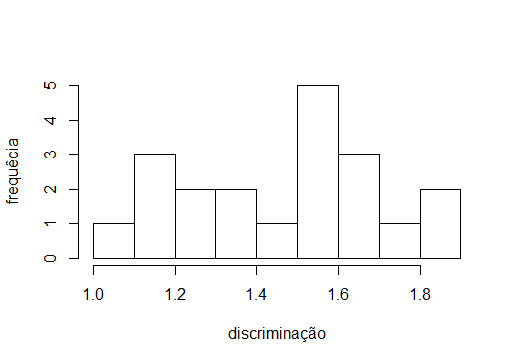
\includegraphics[width=0.6\linewidth]{img/a}
		\caption{}
		\label{fig:a}
	\end{figure}
	
	\newpage
	
	O histograma da figura(\ref{fig:b}) mostra as distribuições para o parâmetro de dificuldade dos 20 itens
	
	\begin{figure}[!h]
		\centering
		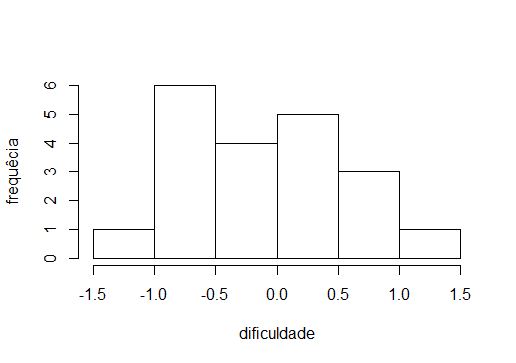
\includegraphics[width=0.6\linewidth]{img/b}
		\caption{}
		\label{fig:b}
	\end{figure}
	
	O histograma da figura(\ref{fig:c})  mostra as distribuições para o parâmetro de acerto ao acaso dos 20 itens.
	\begin{figure}[!h]
		\centering
		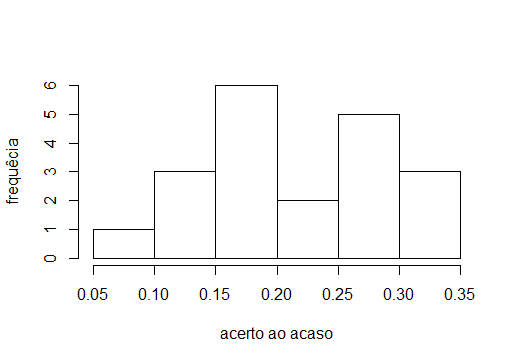
\includegraphics[width=0.6\linewidth]{img/c}
		\caption{}
		\label{fig:c}
	\end{figure}
	\newpage
	O histograma da figura(\ref{fig:hab}) mostra as distribuições para as habilidades dos 20 respondentes.
	\begin{figure} [!h]
		\centering
		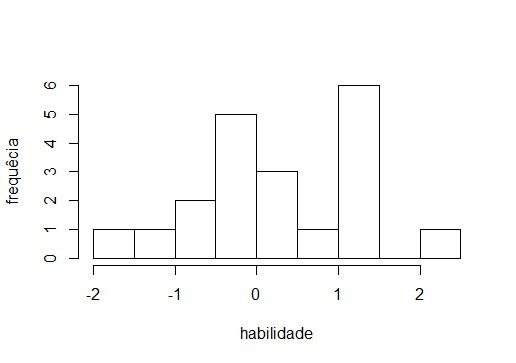
\includegraphics[width=0.6\linewidth]{img/hab}
		\caption{}
		\label{fig:hab}
	\end{figure}
	    A figura(\ref{fig:zeros}) Representa a matriz de zeros e uns, no qual as linhas representam os respondentes e as colunas representam os itens, o valor zero representa que o item foi respondido errado, e um(1) representa que o item foi respondido corretamente. A matriz para 20 respondentes dos 20 alunos(hipotéticos).
    \paragraph{}
		\begin{figure}[!h]
		\caption{Matriz de respostas teste 1}
		\centering
		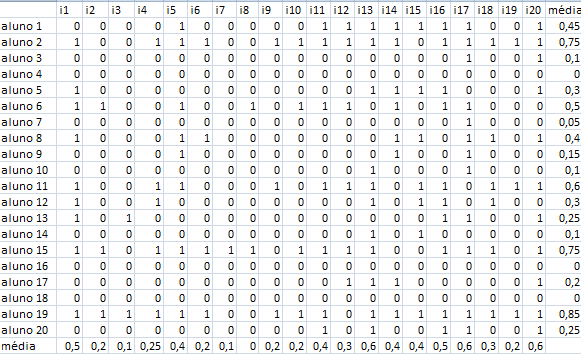
\includegraphics[width=0.6\linewidth]{img/zeros}
		\label{fig:zeros}
	\end{figure}
    Importamos estes dados para o \textit{Excel} e utilizamos o software EIRT\\
 Assim escolhemos para analise o modelo dicotomico de três parâmetros e que estimasse o parâmetros dos itens as habilidades dos alunos hipoteticos.
	A figura(\ref{fig:all_cci}) mostra curva de todos os itens\\
	\paragraph{}
	\begin{figure}
	    \centering
	    \caption{Todas as CCi}
	    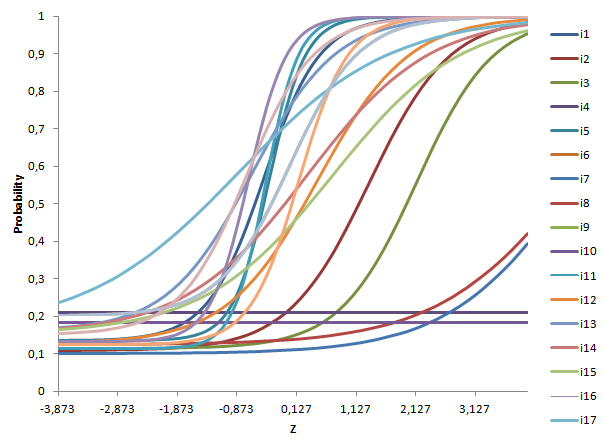
\includegraphics[width=0.5\linewidth]{img/all_cci}
	    \label{fig:all_cci}
	\end{figure}
	    
	Para o teste um alguns itens não convergiram:
	i4,i5,i6,i7,i9,i10,i11 e i19
    Estes itens não convergiram, uma explicação é dada por \textcite{Gleiber}\paragraph{}
   
			\newdimen\mylength
			\mylength = \linewidth
			\addtolength{\mylength}{-4.7cm}
			\hspace{4cm}\begin{minipage}{\mylength}
			    \linespread{1}
				\small{[...] tenta-se manipular os parâmetros do item, produzindo uma curva teórica que mais se aproxime da empírica. O processo de estimação dos parâmetros se encerra quando os valores estimados convergirem, ou seja, quando a partir de n interações não se consegue produzir mais melhorias na reprodução dos dados empíricos por meio das variações nos valores dos parâmetros dos itens. (Wright e Stone, 2004; Baker, 2001; Muñiz, 1990) apud \cite{Gleiber}}
				
			\end{minipage}
		Este fato é facilmente notado através da figura(\ref{fig:all_cci}), o item 1(i4) não se adaptou aos dados, ou seja, a CCI do item 1 não se adaptou a uma curva logística.
   \paragraph{}
   A tabela (\ref{tab:estimacao}) mostra a estimação para os 20 itens.
   \begin{table}[!h]
       \centering
       \begin{tabular}{c|c|c|c}
            \hline
            Item &	Slope (a) &	Threshold (b)&	Asymptote (c)\\
            \hline
            \hline
            i1 &	2,126 &	-0,432 & 0,135 \\
            \hline
            i2 &	1,473 &	1,335 &	0,109 \\
            \hline
            i3 &	1,557 &	2,135 &	0,113 \\
            \hline
            i4 &	0,879 &	12,361 &	0,211 \\
            \hline
            i5 &	3,297 &	-0,334 &	0,136 \\
            \hline
            i6 &	0,884 &	19,457 & 0,184 \\
            \hline
            i7 &	0,949 &	4,770 &	0,102 \\
            \hline
            i8 &	0,868 &	4,784 &	0,126 \\
            \hline
            i9 &	1,702 &	0,000 &	0,200 \\ 
            \hline
            i10 &	0,884 &	18,416 &	0,184 \\
            \hline
            i11 &	3,693 &	-0,396 & 0,115 \\
            \hline
            i12 &	1,313 &	0,477 &	0,128 \\
            \hline
            i13 &	1,424 &	-0,628 &	0,163 \\
            \hline
            i14 &	0,974 &	0,305 & 0,154 \\
            \hline
            i15 &	0,927 &	0,736 &	0,155 \\
            \hline
            i16 &	3,140 &	-0,684 &	0,132 \\
            \hline
            i17 &	0,782 &	-0,856 &	0,166 \\
            \hline
            i18 &	2,444 &	0,160 &	0,126 \\
            \hline
            i19 &	1,702 &	0,000 &	0,200 \\
            \hline
            i20 &	1,775 &	-0,718 &	0,152 \\
            \hline
       \end{tabular}
       \caption{Caption}
       \label{tab:estimacao}
   \end{table}
   \paragraph{}
       A tabela (\ref{tab:habilidadesafter}) mostra as habilidades estimadas para os 20 alunos hipoteticos.
    \begin{table}[!h]
        \centering
        \begin{tabular}{c|c|c|c}
            \hline
            Subject  &	Z	&	Subject	Z\\
            \hline
            \hline
            aluno 1  &	-0,047	&	aluno 11 &	0,750 \\
            \hline
            aluno 2  &	0,918	&	aluno 12 &	-0,784 \\
            \hline
            aluno 3  &	-1,432	&	aluno 13 &	-0,844 \\
            \hline
            aluno 4  &	-1,839	&	aluno 14 &	-1,522 \\
            \hline
            aluno 5  &	-0,633	&	aluno 15 &	0,437 \\
            \hline
            aluno 6  &	-0,142	&	aluno 16 &	-1,839 \\
            \hline
            aluno 7  &	-1,676	&	aluno 17 &	-1,140 \\
            \hline
            aluno 8  &	-0,604	&	aluno 18 &	-1,839 \\
            \hline
            aluno 9  &	-1,403	&	aluno 19 &	1,419 \\
            \hline
            aluno 10 &	-1,471	&	aluno 20 &	-0,601 \\
            \hline
        \end{tabular}
        \caption{Caption}
        \label{tab:habilidadesafter}
    \end{table}
	    
	\paragraph{}
	    Para referência de quais itens são os mais adequados para serem usados em testes Baker( 2001 ) Classifica o parâmetro a da seguinte forma: \\
	\begin{table}[!h]
	    \centering
	    \caption{alguma coisa}
    	\begin{tabular}{|c|c|}
    	    \hline
    	    Muito baixa & de 0,01 a 0,34\\
    	    \hline
    	    Baixa & 0,35 a 0,64\\
    	    \hline
    	    moderada & de 0,64 a 1,34\\
    	    \hline
    	    alta & de 1,35 a 1,69\\
    	    \hline
    	    muito alta & 1,70 \\
    	    \hline
    	\end{tabular}
	\end{table}
	

    \newpage